
	The evaluation goal was to understand what were the main flaws in each system developed by looking at the users difficulties. From its results it was also possible compare the several interaction systems.
	
	For the evaluation test subjects with very different backgrounds, and little technological knowledge were chosen with the exception of one user that had a strong technological understanding. The group of users was composed of men and women, with age from twenty to sixty years old. All of the subjects use a computer every day, although only two users had used \ac{Wiimote} like devices, and none of the users had ever used the Kinect. This was also the first time any of the users interacted with the iCub robot. There was a deliberate choice of users with no technical background because those users do not have any predetermined idea of what to expect from such an interface, or from a humanoid robot. For the evaluation, users were invited to come to the lab during a weekend, so that they could be comfortable.
	
	The evaluation was split into two parts, the tests and the questionnaire. There were six tests made. All of the tests only used the right arm of the iCub, from shoulder to hand. Two of them were based on typical interfaces, a \ac{GUI}, and a \ac{DPad} (the \ac{Wiimote} cursor). The other four were based on two novel interfaces, the \ac{Wiimote}, and the Kinect. The novel devices interfaces were used in two tests each, one using individual motor control, the \ac{Wiimote} motor test, and the Kinect skeleton test, and the other on the Cartesian control, the \ac{Wiimote} kinematic test, and the Kinect hand kinematic test. For the tests there was no feedback other than the robot reaction, this made the tests harder. Using a graphical feedback would result on having to consider the design of that feedback and not only the interaction allowed by the interface. These tests followed the interaction described in section \ref{sec:interface}, and used the applications described in section \ref{sec:application}.
	
	Before and during the tests a presentation was shown describing what was the iCub project, what was the goal of that evaluation, what should the test subjects do, and how the interfaces worked.
	
	The tests were divided into five tasks. The three first tasks of the tests were made to make the user comfortable, and to check if the user was able to do the most basic tasks. The first task was to ``play around'' with the interface, the second task was to move the arm up and down, the third task was to move the arm left and right. All users successfully conclude these tasks without any difficulty.
	
	The fourth and fifth tasks used a set of four objects placed at the right arm reach distance and suspended from the ceiling. The objects were numbered from one to four, as can be seen in Fig.\ref{fig:icubTestScenary}. For this tasks the time spent, the amount of errors and the user comments were annotated. Before any of the tasks started the robot arm was positioned into an initial ``safe'' position.
	
	\begin{figure}[htb]
	\centering
	  \subfloat[Front view.]{\label{fig:icubTestSceneryFront}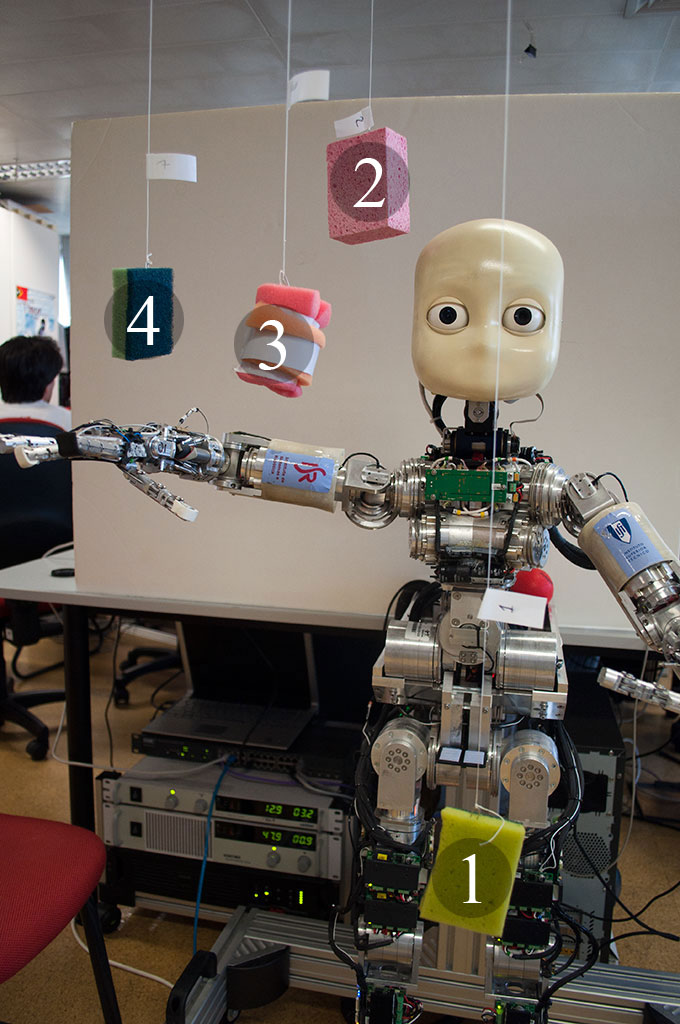
\includegraphics[width=32mm]{testSceneryFront.jpg}}
  \hspace{5mm}
	  \subfloat[Left view.]{\label{fig:icubTestSceneryLeft}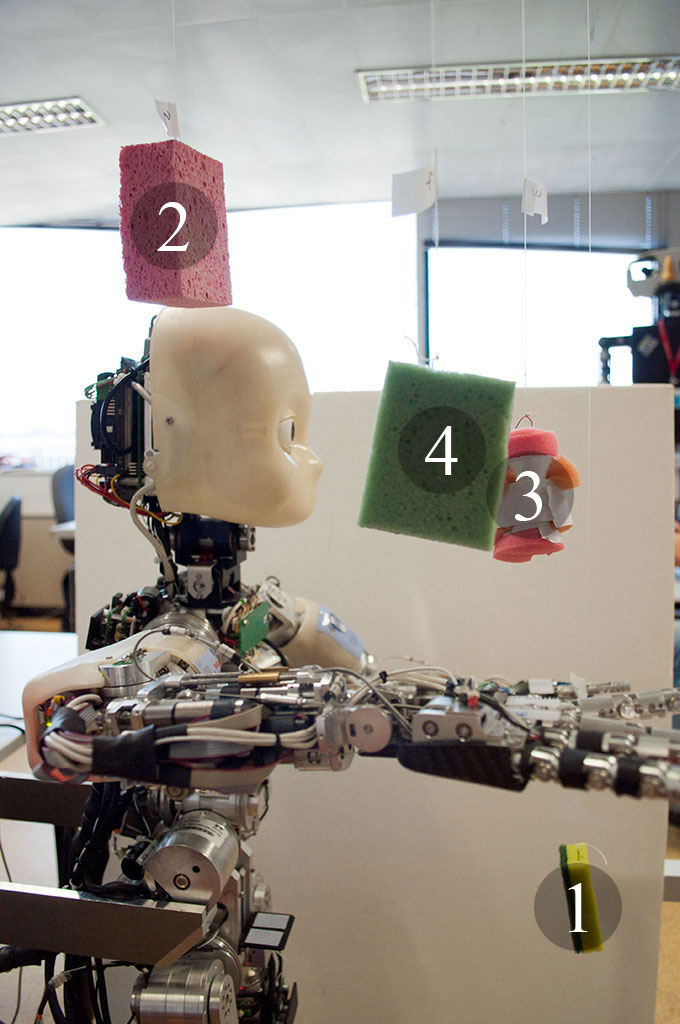
\includegraphics[width=32mm]{testSceneryLeft.jpg}}
	\caption[Interfaces test scenery]{Interfaces test scenery.} 
	\label{fig:icubTestScenary}
	\end{figure}
	
	The goal of task four was to touch all the objects, from one to four, without colliding with any of the other objects if possible. The goal of task five was to touch objects four one and two, by this order. But in task five besides not colliding with the unintended objects, there was an obstacle (an A4 sheet of paper), placed in the object three position. Collision with the obstacle should be avoided. Figures \ref{fig:tasksResults} shows the amount of time needed to conclude the tasks, and the amount of errors per task.
	
	\begin{figure}[htb]
	\centering
	  \subfloat[Task time comparison.]{\label{fig:taskTimeCompare}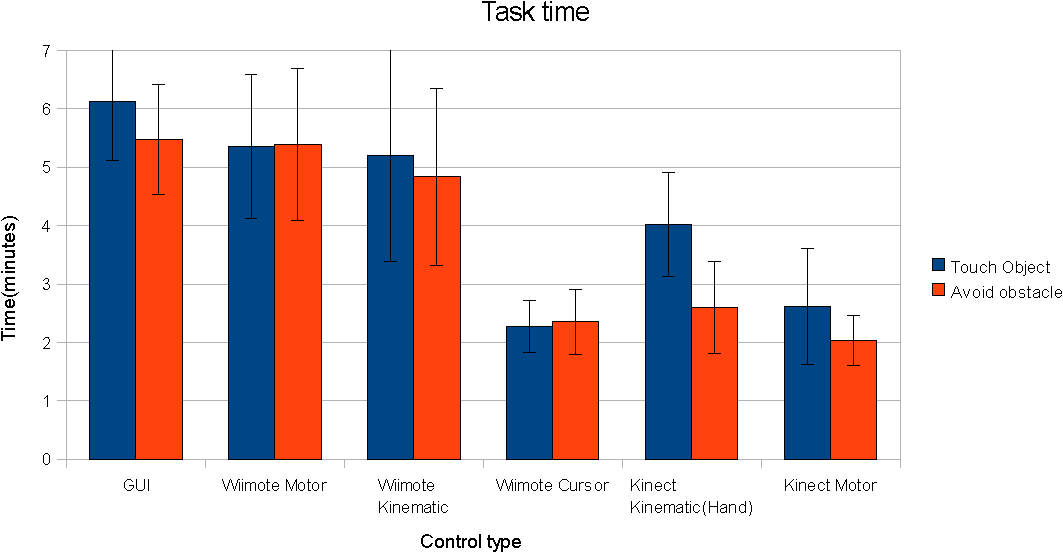
\includegraphics[width=70mm,page=1]{graphsPDF-crop.pdf}}
  \hspace{5mm}
	  \subfloat[Task error comparison.]{\label{fig:taskErrorCompare}\includegraphics[width=70mm,page=2]{graphsPDF-crop.pdf}}
	  \caption{Tasks results.}
	  \label{fig:tasksResults}
	\end{figure}

	The graphs support the idea that the most successful interaction was the \ac{Wiimote} cursor. The \ac{DPad} interface is the one that got the best time and smaller error values. From user comments it was possible to understand that this interface was the most well known by users, helping to visualize how action with the interface would result in a robot reaction. By contrast the Kinect interface was the least known interface. Although when comparing the Kinect interface performance with the \ac{DPad} interface performance, the results were very similar in number of errors and amount of time. The \ac{GUI} interface was a classic interface, but the control of the robot was considered too complicated by the users, even with only three sliders. 
	 The \ac{Wiimote} interactions were the most difficult to make the user understand how the interaction worked. That difficulty in understanding was reflected into the results. It is assumed that the understanding of how the interaction works is related to the difficulty of control. One of the subjects achieved very good results in the \ac{Wiimote} motor interface only after being extremely clear about how the interaction worked. This interface was specially bad with the older users that did not seem to be comfortable with the explanation.
